% Document Class is specified here. We're using the Homework Template
\documentclass[12pt, a4paper]{article}

\usepackage{graphicx}
\usepackage{float}
\usepackage{geometry}
\usepackage{verbatim}
\usepackage{listings}

\lstset{
  basicstyle=\itshape,
  xleftmargin=3em,
  literate={->}{$\rightarrow$}{2}
           {ε}{$\epsilon$}{1}
}

\geometry{a4paper, margin=1in}

\title{Week 9 CS-312 Homework}
\author{
	Cory Ness
	\and
	Jack Engledow
	\and
	James Sgrazzutti
}

\begin{document}

\maketitle

\section{Problem 11.5}
\subsection{Question}
Draw the diagram for a TM that accepts $\{0^{a}1^{b}: a < b\}$.
\subsection{Answer}
\begin{center}
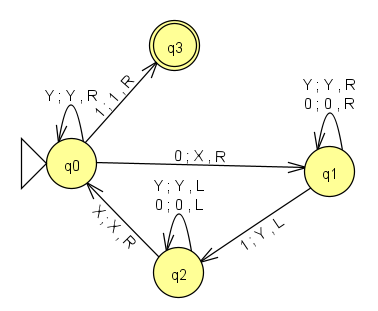
\includegraphics[scale=1]{11.5}
\end{center}

\section{Problem 11.7}
\subsection{Question}
Draw the diagram for a TM that accepts $\{a^{2^{n}}: n > 0\}$.
\subsection{Answer}
\begin{center}
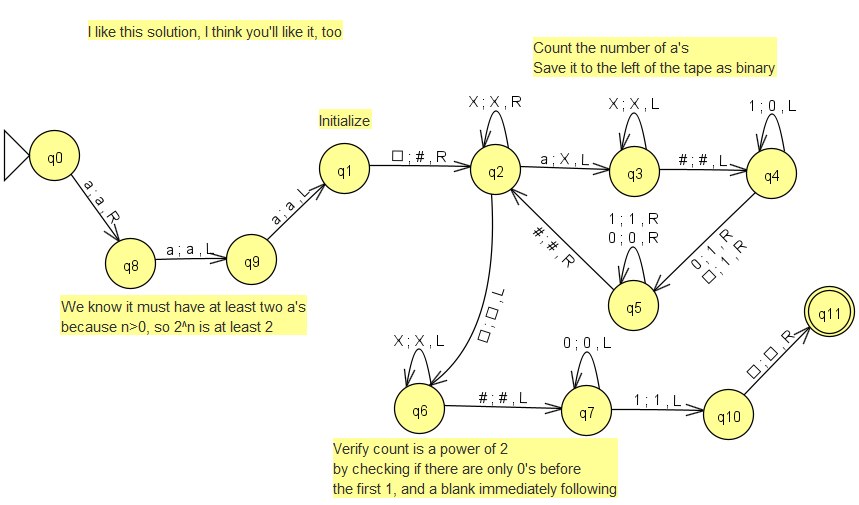
\includegraphics[scale=0.8]{11.7}
\end{center}

\section{Problem 11.17}
\subsection{Question}
Describe a TM subroutine that effectively deletes a symbol; that is, it deletes the symbol and shifts left all symbols to the right of this point.
\subsection{Answer}
The subroutine is defined as entering at the location of the symbol to delete, and follows the general format below, where there is a branch for every possible character of the tape alphabet.
\begin{center}
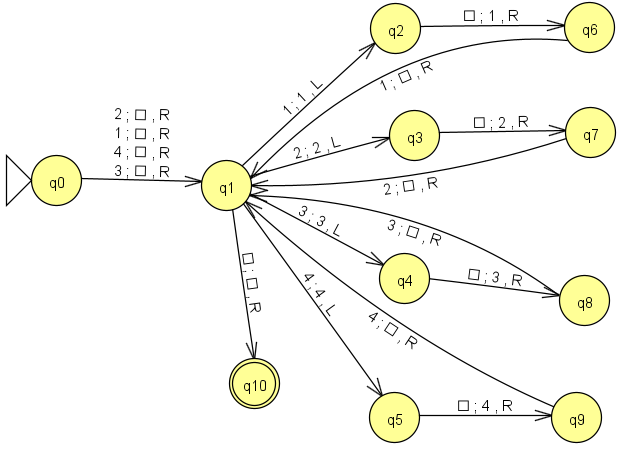
\includegraphics[scale=1]{11.17}
\end{center}

\section{Problem 12.3c}
\subsection{Question}
Write a TM that treat the input as a unary number and computes the remainder when the input is divided by 3.
\subsection{Answer}
Assuming that computed number is to be placed at the end of the unary number and that the symbol "a" will represent the unary symbol...
\begin{center}
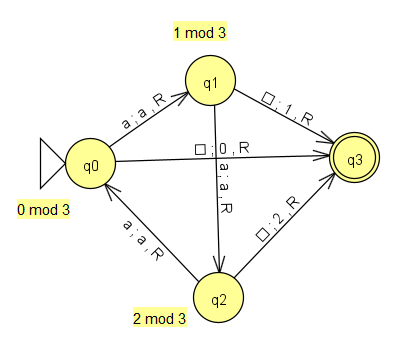
\includegraphics[scale=1]{12.3c}
\end{center}

\section{Problem 12.15}
\subsection{Question}
Suppose you have a TM $M$ for language $L$. Describe in English how to build a nondeterministic TM for language $L^{*}$.
\subsection{Answer}
First take $M$ and turn it into a nondeterministic TM by connecting all final states to a new final state via a $\epsilon; \epsilon, N$ (where N represents no movement) transition. Then, treat that new NTM as a subroutine where it enters at the initialization state and exits at the final state. We can create a new NTM similarly to creating a new NFA that supports the kleene star operation, but with the exception that instead of the "end" state being a final state, it instead allows a transition to a final state via a $\Delta; \Delta, R$ transition, with the $\Delta$s represented by "O"s in the picture below.
\begin{center}
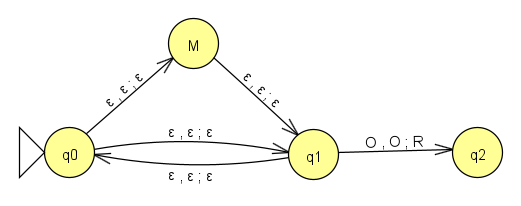
\includegraphics[scale=1]{12.15}
\end{center}

\section{Problem 12.19}
\subsection{Question}
Sometimes a TM is defined to have a one-way infinite tape. The input is written at the start of the tape. The machine crashes if it tries to move off the left end of the tape.\newline
Sketch how to convert a program that runs on the standard TM model to that model, and vice versa.
\subsection{Answer}
We can easily turn a one-way infinite tape TM to a standard TM by doing nothing, as a one-way infinite tape TM will operate perfectly fine on a two-way infinite TM.\newline
\newline
We can also turn a standard TM into a one-way infinite tape TM by following these instructions.\newline
 1. Add a special symbol $@$ that represents the start of the tape\newline
 2. Change the input string to instead be on every nth position of the tape, instead be on every 2n position of the tape. For example the 1st symbol is on the 2nd position, 2nd symbol on the 4th position, etc.\newline
 3. Keep track of a binary state called "signage", which initializes to "positive"\newline
And for every transition (found by performing a graph search of all nodes), follow these instructions.\newline
 4. If moving to the right while "positive", instead move to the right twice.\newline
 5. If moving to the left while "positive", instead move to the left twice.\newline
 6. If moving to the right while "negative", instead move to the left twice.\newline
 7. If moving to the left while "negative", instead move to the right twice.\newline
 8. If, while moving, you encounter the special symbol $@$, and the state is "negative" (you have moved twice), the state is now positive, move to the right by one.\newline
 9. If, while moving, you encounter the special symbol $@$, and the state is "positive" (you have moved once), the state is now "negative", move to the right by two.\newline
\newline
Following these steps, the new turing machine will place all symbols that would lie on the positive end of the two-way tape on every even slot, and the negative symbols on the two-way tape on every odd slot (with -0 being taken up by the special symbol).

\section{Problem 13.1}
\subsection{Question}
Let $M$ be an FA and $q$ some state of $M$. Call $q$ a useful state if there exists some input $w$ such that $M$ actually enters $q$. Let $B = \{<M,q>:q$ is a useful state of $M \}$. Show that $B$ is recursive.
\subsection{Answer}
Without loss of generality, assume $M$ is a DFA, if it is not, convert $M$ into a DFA. Since $M$ is now a DFA, simulate $M$ on $q$. Since $M$ is a DFA, it will eventually halt, thus $M$ is recursive.

\section{Problem 13.14}
\subsection{Question}
Show that if $L$ is accepted by a nondeterministic TM that always halts, then $L$ is recursive.
\subsection{Answer}
Simulate that nondeterministic TM by deterministic TM $M$, and if a branch crashes, continue, otherwise if a branch halts, halt $M$. Since the nondeterministic TM will eventually halt, that means $M$ will eventually halt, and since $M$ halts on $L$, $L$ is recursive.

\section{Problem 13.18}
\subsection{Question}
Let language $Right_{tm} = \{<M,w>: M$ is a TM that when started on input $w$ never moves its head left $\}$.
\subsubsection{Compute a quantity $Q$ such that, if $M$ runs for longer than this time on $w$ without moving its head left, then it will run forever.}
If there is a Turing machine that never moves to the left, it is unable to access memory, and is equal to a Finite Automata that also acts on empty symbols. Thus, create a Finite Automata that acts on empty symbols, and $Q = |input| + |states|$. This is because after $|input|$ transitions have passed, the FA must be acting solely on empty symbols, and after $|states|$ transitions have passed, at least one state must have been reached twice, due to the pigeon hole principle. This means there is a loop consisting entirely of transitions that act only on empty symbols, and there are only empty symbols left in the tape, thus the FA will run forever.
\subsubsection{Use this to show that $Right_{tm}$ is recursive.}
Because there is a modified FA that is equivalent to $M$ where it is known when it will run forever, $Right_{tm}$ can be created to simulate the FA. In the case that the FA halts, the TM halts. If the FA does not halt and passes $Q$, the TM can recognize this and halt, rejecting the input. Because the TM can halt in either case of the FA, the TM $Right_{tm}$ is Recursive.

\end{document}